\documentclass[journal,10pt,twocolumn]{IEEEtran} 

\usepackage{amssymb}
\usepackage{amsthm} % 包含定理、命题、引理等环境
\usepackage{multirow}
\usepackage{booktabs}
\usepackage{longtable}
\usepackage{amsfonts}
\usepackage{ltablex}
\keepXColumns
\usepackage{wrapfig}
\usepackage{subcaption}
%\usepackage{subfigure}
\usepackage{algorithmic,algorithm}
\usepackage{color, soul}
\ifCLASSINFOpdf
   \usepackage[pdftex]{graphicx}
  \graphicspath{{../pdf/}{../jpeg/}}
   \DeclareGraphicsExtensions{.pdf,.jpeg,.png}
\else
  \usepackage[dvips]{graphicx}
   \graphicspath{{../eps/}}
   \DeclareGraphicsExtensions{.eps}
\fi
\usepackage{cite}
\usepackage{amsmath}
\usepackage{array}
\usepackage{epstopdf}
\usepackage{extarrows}
% added by shuai wang
% the commands defined for ease of usage
\usepackage{hyperref}
\usepackage{multirow}
\usepackage{bm}  %可使用\bm命令进行加粗
\usepackage[table]{xcolor}
\usepackage{pifont}% http://ctan.org/pkg/pifont
\usepackage{supertabular}
\usepackage{scalerel}
\usepackage{float} 
\usepackage{xcolor}
\usepackage{tabularx}
\newcommand{\cmark}{\ding{51}}%
\newcommand{\xmark}{\ding{55}}%


%手写体
\newcommand\AC{\ensuremath{\mathcal{A}}}
\newcommand\BC{\ensuremath{\mathcal{B}}}
\newcommand\CC{\ensuremath{\mathcal{C}}}
\newcommand\DC{\ensuremath{\mathcal{D}}}
\newcommand\EC{\ensuremath{\mathcal{E}}}
\newcommand\FC{\ensuremath{\mathcal{F}}}
\newcommand\GC{\ensuremath{\mathcal{G}}}
\newcommand\HC{\ensuremath{\mathcal{H}}}
\newcommand\IC{\ensuremath{\mathcal{I}}}
\newcommand\JC{\ensuremath{\mathcal{J}}}
\newcommand\KC{\ensuremath{\mathcal{K}}}
\newcommand\LC{\ensuremath{\mathcal{L}}}
\newcommand\MC{\ensuremath{\mathcal{M}}}
\newcommand\NC{\ensuremath{\mathcal{N}}}
\newcommand\OC{\ensuremath{\mathcal{O}}}
\newcommand\PC{\ensuremath{\mathcal{P}}}
\newcommand\QC{\ensuremath{\mathcal{Q}}}
\newcommand\RC{\ensuremath{\mathcal{R}}}
\newcommand\SC{\ensuremath{\mathcal{S}}}
\newcommand\TC{\ensuremath{\mathcal{T}}}
\newcommand\UC{\ensuremath{\mathcal{U}}}
\newcommand\VC{\ensuremath{\mathcal{V}}}
\newcommand\WC{\ensuremath{\mathcal{W}}}
\newcommand\XC{\ensuremath{\mathcal{X}}}
\newcommand\YC{\ensuremath{\mathcal{Y}}}
\newcommand\ZC{\ensuremath{\mathcal{Z}}}

%数学符号加粗体(文字加粗可用\bf)
\newcommand\AB{\ensuremath{\bm{A}}}
\newcommand\BB{\ensuremath{\bm{B}}}
\newcommand\CB{\ensuremath{\bm{C}}}
\newcommand\DB{\ensuremath{\bm{D}}}
\newcommand\EB{\ensuremath{\bm{E}}}
\newcommand\FB{\ensuremath{\bm{F}}}
\newcommand\GB{\ensuremath{\bm{G}}}
\newcommand\HB{\ensuremath{\bm{H}}}
\newcommand\IB{\ensuremath{\bm{I}}}
\newcommand\JB{\ensuremath{\bm{J}}}
\newcommand\KB{\ensuremath{\bm{K}}}
\newcommand\LB{\ensuremath{\bm{L}}}
\newcommand\MB{\ensuremath{\bm{M}}}
\newcommand\NB{\ensuremath{\bm{N}}}
\newcommand\OB{\ensuremath{\bm{O}}}
\newcommand\PB{\ensuremath{\bm{P}}}
\newcommand\QB{\ensuremath{\bm{Q}}}
\newcommand\RB{\ensuremath{\bm{R}}}
\newcommand\SB{\ensuremath{\bm{S}}}
\newcommand\TB{\ensuremath{\bm{T}}}
\newcommand\UB{\ensuremath{\bm{U}}}
\newcommand\VB{\ensuremath{\bm{V}}}
\newcommand\WB{\ensuremath{\bm{W}}}
\newcommand\XB{\ensuremath{\bm{X}}}
\newcommand\YB{\ensuremath{\bm{Y}}}
\newcommand\ZB{\ensuremath{\bm{Z}}}

\newcommand\aB{\ensuremath{\bm{a}}}
\newcommand\bB{\ensuremath{\bm{b}}}
\newcommand\cB{\ensuremath{\bm{c}}}
\newcommand\dB{\ensuremath{\bm{d}}}
\newcommand\eB{\ensuremath{\bm{e}}}
\newcommand\fB{\ensuremath{\bm{f}}}
\newcommand\gB{\ensuremath{\bm{g}}}
\newcommand\hB{\ensuremath{\bm{h}}}
\newcommand\iB{\ensuremath{\bm{i}}}
\newcommand\jB{\ensuremath{\bm{j}}}
\newcommand\kB{\ensuremath{\bm{k}}}
\newcommand\lB{\ensuremath{\bm{l}}}
\newcommand\mB{\ensuremath{\bm{m}}}
\newcommand\nB{\ensuremath{\bm{n}}}
\newcommand\oB{\ensuremath{\bm{o}}}
\newcommand\pB{\ensuremath{\bm{p}}}
\newcommand\qB{\ensuremath{\bm{q}}}
\newcommand\rB{\ensuremath{\bm{r}}}
\newcommand\sB{\ensuremath{\bm{s}}}
\newcommand\tB{\ensuremath{\bm{t}}}
\newcommand\uB{\ensuremath{\bm{u}}}
\newcommand\vB{\ensuremath{\bm{v}}}
\newcommand\wB{\ensuremath{\bm{w}}}
\newcommand\xB{\ensuremath{\bm{x}}}
\newcommand\yB{\ensuremath{\bm{y}}}
\newcommand\zB{\ensuremath{\bm{z}}}

\newcommand\muB{\ensuremath{{\bm \mu}}}
\newcommand\betaB{\ensuremath{{\bm \beta}}}
\newcommand\gammaB{\ensuremath{{\bm \gamma}}}
\newcommand\thetaB{\ensuremath{{\bm \theta}}}
\newcommand\nuB{\ensuremath{{\bm \nu}}}
\newcommand\lambdaB{\ensuremath{{\bm \lambda}}}
\newcommand\OmegaB{\ensuremath{{\bm \Omega}}}
\newcommand\omegaB{\ensuremath{{\bm \omega}}}
\newcommand\UpsilonB{\ensuremath{{\bm \Upsilon}}}
\newcommand\zeroB{\ensuremath{{\bm 0}}}
\newcommand\etaB{\ensuremath{{\bm \eta}}}
\newcommand\xiB{\ensuremath{{\bm \xi}}}
\newcommand\psiB{\ensuremath{{\bm \psi}}}
\newcommand\PsiB{\ensuremath{{\bm \Psi}}}
\newcommand\phiB{\ensuremath{{\bm \phi}}}
\newcommand\sigmaB{\ensuremath{{\bm \sigma}}}
\newcommand\piB{\ensuremath{{\bm \pi}}}



%数学符号加正粗体
\newcommand\AF{\ensuremath{\mathbf{A}}}
\newcommand\BF{\ensuremath{\mathbf{B}}}
\newcommand\CF{\ensuremath{\mathbf{C}}}
\newcommand\DF{\ensuremath{\mathbf{D}}}
\newcommand\EF{\ensuremath{\mathbf{E}}}
\newcommand\FF{\ensuremath{\mathbf{F}}}
\newcommand\GF{\ensuremath{\mathbf{G}}}
\newcommand\HF{\ensuremath{\mathbf{H}}}
\newcommand\FIF{\ensuremath{\mathbf{I}}}
\newcommand\JF{\ensuremath{\mathbf{J}}}
\newcommand\KF{\ensuremath{\mathbf{K}}}
\newcommand\LF{\ensuremath{\mathbf{L}}}
\newcommand\MF{\ensuremath{\mathbf{M}}}
\newcommand\NF{\ensuremath{\mathbf{N}}}
\newcommand\OF{\ensuremath{\mathbf{O}}}
\newcommand\PF{\ensuremath{\mathbf{P}}}
\newcommand\QF{\ensuremath{\mathbf{Q}}}
\newcommand\RF{\ensuremath{\mathbf{R}}}
\newcommand\SF{\ensuremath{\mathbf{S}}}
\newcommand\TF{\ensuremath{\mathbf{T}}}
\newcommand\UF{\ensuremath{\mathbf{U}}}
\newcommand\VF{\ensuremath{\mathbf{V}}}
\newcommand\WF{\ensuremath{\mathbf{W}}}
\newcommand\XF{\ensuremath{\mathbf{X}}}
\newcommand\YF{\ensuremath{\mathbf{Y}}}
\newcommand\ZF{\ensuremath{\mathbf{Z}}}


\newcommand\muF{\ensuremath{{\mathbf \mu}}}
\newcommand\betaF{\ensuremath{{\mathbf \beta}}}
\newcommand\gammaF{\ensuremath{{\mathbf \gamma}}}
\newcommand\thetaF{\ensuremath{{\mathbf \theta}}}
\newcommand\nuF{\ensuremath{{\mathbf \nu}}}
\newcommand\lambdaF{\ensuremath{{\mathbf \lambda}}}
\newcommand\OmegaF{\ensuremath{{\mathbf \Omega}}}
\newcommand\omegaF{\ensuremath{{\mathbf \omega}}}
\newcommand\UpsilonF{\ensuremath{{\mathbf \Upsilon}}}
\newcommand\zeroF{\ensuremath{{\mathbf 0}}}
\newcommand\oneF{\ensuremath{{\mathbf 1}}}
\newcommand\etaF{\ensuremath{{\mathbf \eta}}}
\newcommand\xiF{\ensuremath{{\mathbf \xi}}}
\newcommand\psiF{\ensuremath{{\mathbf \psi}}}
\newcommand\PsiF{\ensuremath{{\mathbf \Psi}}}
\newcommand\phiF{\ensuremath{{\mathbf \phi}}}
\newcommand\sigmaF{\ensuremath{{\mathbf \sigma}}}
\newcommand\piF{\ensuremath{{\mathbf \pi}}}


%数学符号正体
\newcommand\AR{\ensuremath{\mathrm{A}}}
\newcommand\BR{\ensuremath{\mathrm{B}}}
\newcommand\CR{\ensuremath{\mathrm{C}}}
\newcommand\DR{\ensuremath{\mathrm{D}}}
\newcommand\ER{\ensuremath{\mathrm{E}}}
\newcommand\FR{\ensuremath{\mathrm{F}}}
\newcommand\GR{\ensuremath{\mathrm{G}}}
\newcommand\HR{\ensuremath{\mathrm{H}}}
\newcommand\IR{\ensuremath{\mathrm{I}}}
\newcommand\JR{\ensuremath{\mathrm{J}}}
\newcommand\KR{\ensuremath{\mathrm{K}}}
\newcommand\LR{\ensuremath{\mathrm{L}}}
\newcommand\MR{\ensuremath{\mathrm{M}}}
\newcommand\NR{\ensuremath{\mathrm{N}}}
\newcommand\ROR{\ensuremath{\mathrm{O}}}
\newcommand\PR{\ensuremath{\mathrm{P}}}
\newcommand\QR{\ensuremath{\mathrm{Q}}}
\newcommand\RR{\ensuremath{\mathrm{R}}}
\newcommand\SR{\ensuremath{\mathrm{S}}}
\newcommand\TR{\ensuremath{\mathrm{T}}}
\newcommand\UR{\ensuremath{\mathrm{U}}}
\newcommand\VR{\ensuremath{\mathrm{V}}}
\newcommand\WR{\ensuremath{\mathrm{W}}}
\newcommand\XR{\ensuremath{\mathrm{X}}}
\newcommand\YR{\ensuremath{\mathrm{Y}}}
\newcommand\ZR{\ensuremath{\mathrm{Z}}}

\newcommand\aR{\ensuremath{\mathrm{a}}}
\newcommand\bR{\ensuremath{\mathrm{b}}}
\newcommand\cR{\ensuremath{\mathrm{c}}}
\newcommand\dR{\ensuremath{\mathrm{d}}}
\newcommand\eR{\ensuremath{\mathrm{e}}}
\newcommand\fR{\ensuremath{\mathrm{f}}}
\newcommand\gR{\ensuremath{\mathrm{g}}}
\newcommand\hR{\ensuremath{\mathrm{h}}}
\newcommand\iR{\ensuremath{\mathrm{i}}}
\newcommand\jR{\ensuremath{\mathrm{j}}}
\newcommand\kR{\ensuremath{\mathrm{k}}}
\newcommand\lR{\ensuremath{\mathrm{l}}}
\newcommand\mR{\ensuremath{\mathrm{m}}}
\newcommand\nR{\ensuremath{\mathrm{n}}}
\newcommand\RoR{\ensuremath{\mathrm{o}}}
\newcommand\pR{\ensuremath{\mathrm{p}}}
\newcommand\qR{\ensuremath{\mathrm{q}}}
\newcommand\rR{\ensuremath{\mathrm{r}}}
\newcommand\sR{\ensuremath{\mathrm{s}}}
\newcommand\tR{\ensuremath{\mathrm{t}}}
\newcommand\uR{\ensuremath{\mathrm{u}}}
\newcommand\vR{\ensuremath{\mathrm{v}}}
\newcommand\wR{\ensuremath{\mathrm{w}}}
\newcommand\xR{\ensuremath{\mathrm{x}}}
\newcommand\yR{\ensuremath{\mathrm{y}}}
\newcommand\zR{\ensuremath{\mathrm{z}}}
\newcommand\zeroR{\ensuremath{\mathrm{0}}}

\newcommand\rank{\ensuremath{\mathrm{rank}}}
\newcommand\SNR{\ensuremath{\mathrm{SNR}}}
%\newcommand\st{\ensuremath{\mathrm{s.t.}}}
\newcommand\RSS{\ensuremath{\mathrm{RSS}}}
\newcommand\des{\ensuremath{\mathrm{des}}}
\newcommand\OCC{\ensuremath{\mathrm{OCC}}}
\newcommand\MSE{\ensuremath{\mathrm{MSE}}}
\newcommand\ENS{\ensuremath{\mathrm{ENS}}}
\newcommand\MO{\ensuremath{\mathrm{MO}}}
\newcommand\sign{\ensuremath{\mathrm{sign}}}
\newcommand\Conv{\ensuremath{\mathrm{Conv}}}
\newcommand\sigmoid{\ensuremath{\mathrm{sigmoid}}}
\newcommand\stack{\ensuremath{\mathrm{stack}}}
\newcommand\Gen{\ensuremath{\mathrm{Gen}}}
\newcommand\Dis{\ensuremath{\mathrm{Dis}}}
\newcommand\Pen{\ensuremath{\mathrm{Pen}}}
\newcommand\rx{\ensuremath{\mathrm{rx}}}
\newcommand\tx{\ensuremath{\mathrm{tx}}}
\newcommand\BS{\ensuremath{\mathrm{BS}}}
\newcommand\corr{\ensuremath{\mathrm{corr}}}
\newcommand\smax{\ensuremath{\mathrm{smax}}}
\newcommand\smin{\ensuremath{\mathrm{smin}}}
\newcommand\ReLU{\ensuremath{\mathrm{ReLU}}}
\newcommand\CE{\ensuremath{\mathrm{CE}}}

\newcommand\thetaR{\ensuremath{{\mathrm{\theta}}}}

%空心粗体

\newcommand\Cb{\ensuremath{\mathbb{C}}}
\newcommand\Eb{\ensuremath{\mathbb{E}}}
\newcommand\Hb{\ensuremath{\mathbb{H}}}
\newcommand\Ib{\ensuremath{\mathbb{I}}}
\newcommand\Rb{\ensuremath{\mathbb{R}}}
\newcommand\Zb{\ensuremath{\mathbb{Z}}}




% Attempt to make hyperref and algorithmic work together better:
%\newcommand{\theHalgorithm}{\arabic{algorithm}}
\newcommand{\dataset}{{\cal D}}
\newcommand{\fracpartial}[2]{\frac{\partial #1}{\partial  #2}}


\newcommand{\wt}{\widetilde}
\newcommand{\wh}{\widehat}
\newcommand{\ol}{\overline}
%\newcommand{\ul}{\underline}

\newtheorem{Lemma}{Lemma}
\newtheorem{Prop}{Proposition}
\newtheorem{Theorem}{Theorem}
\newtheorem{Def}{Definition}
\newtheorem{Corollary}{Corollary}
\newtheorem{Property}{Property}
\newtheorem{Exa}{Example}
\newtheorem{Rmk}{Remark}
\newtheorem{assumption}{Assumption}

\def\red{\color{red}}
\def\balck{\color{black}}
\def\blue{\color{blue}}
\def\green{\color{green}}

\usepackage{acronym}
\newacro{isac}[ISAC]{integrated sensing and communication}
\newacro{rss}[RSS]{received signal strength}
\newacro{cgan}[CGAN]{conditional generative adversarial network}
\newacro{thz}[THz]{terahertz}
\newacro{sota}[SOTA]{state-of-the-art}
\newacro{mse}[MSE]{mean squared error}
\newacro{dl}[DL]{deep learning}
\newcommand{\tabincell}[2]{\begin{tabular}{@{}#1@{}}#2\end{tabular}}
\newacro{pdf}[PDF]{probability density function}
\newacro{bs}[BS]{base station}
\newacro{awgn}[AWGN]{additive white Gaussian noise}
\newacro{ssb}[SSB]{synchronization
signal blocks}
\newacro{ssb}[SSB]{synchronization
signal blocks}
\newacro{dod}[DoD]{directions of departure}
\newacro{dnn}[DNN]{deep neural network}
\newacro{gan}[GAN]{generative adversarial network}
\newacro{cnn}[CNN]{convolutional neural network}


\newtheorem{proposition}{Proposition}
\renewcommand{\qedsymbol}{$\blacksquare$}
\hyphenation{op-tical net-works semi-conduc-tor}

% \setlength\floatsep{0.2\baselineskip plus 3pt minus 2pt}
% \setlength\textfloatsep{0.2\baselineskip plus 3pt minus 2pt}
% \setlength\intextsep{0.2\baselineskip plus 3pt minus 2pt}
% \setlength{\abovecaptionskip}{0.05cm}
% \setlength{\belowcaptionskip}{0.05cm}

% \usepackage[explicit]{titlesec}
% \titlespacing*{\section}{0pt}{1.2ex plus .0ex minus .0ex}{.8ex plus .0ex}
% \titlespacing*{\subsection}{0pt}{1.5ex plus .0ex minus .0ex}{1.0ex plus .0ex}

% \setlength{\textfloatsep}{8pt}   % figure 与正文之间的距离
% \setlength{\floatsep}{8pt}       % 两个浮动体之间的距离
% \makeatletter
% \setlength{\@fptop}{0pt}
% \makeatother

\begin{document}

\title{\LARGE Channel Gains to Captions: Task-Unified Multi-Level RF Sensing with Vision-Language Models}
%signal strength； propagation field ；sensor-bound radio measurements；Channel Knowledge Map 
\author{Tianyu~Hu,~\IEEEmembership{Student Member,~IEEE,} Zhiren~Gong,~\IEEEmembership{Student Member,~IEEE,}
        Haowei~Cui, Shuai~Wang,~\IEEEmembership{Member,~IEEE,} Samson~Lasaulce,~\IEEEmembership{Member,~IEEE,} Lingxiang~Li,~\IEEEmembership{Member,~IEEE,} Wassim~Hamidouche,~\IEEEmembership{Senior Member,~IEEE,}  
        Zhi~Chen,~\IEEEmembership{Senior Member,~IEEE,} \text{Mérouane}~Debbah,~\IEEEmembership{Fellow,~IEEE}
    \thanks{This work is supported in part by Mobile Information Networks-National Science and Technology Major Project under Grant No. 2025ZD1305200, and by the National Key R\&D Program of China under Grant 2024YFE0200400. (Corresponding authors: Lingxiang Li and Shuai Wang)}
    \thanks{Tianyu Hu, Haowei Cui, Shuai Wang, Lingxiang Li, and Zhi Chen are with the National Key Laboratory of Wireless Communications, University of Electronic Science and Technology of China (UESTC), Chengdu 611731, China (e-mail: \{huty, cchw\}@std.uestc.edu.cn; \{shuaiwang, lingxiang.li, chenzhi\}@uestc.edu.cn;).}
    \thanks{Zhiren Gong is with the Interdisciplinary Graduate Programme, Nanyang Technological University, Singapore (e-mail: zhiren001@e.ntu.edu.sg).}
    \thanks{Tianyu Hu, Samson Lasaulce, Wassim~Hamidouche, and \text{Mérouane} Debbah are with the Research Institute for Digital Future, Khalifa University, 127788 Abu Dhabi, UAE (e-mail: huty@std.uestc.edu.cn, \{wassim.hamidouche, samson.lasaulce,merouane.debbah\}@ku.ac.ae).}
}
\IEEEaftertitletext{\vspace{-1.5\baselineskip}}
\maketitle

\begin{abstract}
This letter investigates a task-unified multi-level radio-frequency (RF) sensing framework driven by vision–language models (VLMs). Existing RF sensing methods rely on task-specific designs and provide only partial environmental information, limiting their ability to handle emerging 6G applications. To address this, we formulate the RF sensing problem as a captioning task, mapping millimeter-wave (mmWave)/terahertz (THz) channel gains to captions describing multi-level environmental semantics. The framework solves this problem by fine-tuning a VLM, leveraging its knowledge-rich multimodal representations and prompt-conditioned semantic generation capabilities. Hence, different sensing tasks are specified through textual prompts, enabling the framework to handle diverse tasks in a unified manner. For fine-tuning, we introduce prompt-routed low-rank adaptation (LoRA) experts to achieve level-aware adaptation, thereby mitigating the discrepancy between propagation characteristics and visual–textual priors. Simulation results show that the proposed framework achieves up to 0.31 improvement in F1 score over the baselines, indicating better sensing performance in terms of precision and recall.



\end{abstract}

\begin{IEEEkeywords}
RF sensing, multi-level environmental semantics, task-unified model, VLMs, mmWave/THz channel gains.
% 我看你后文写的vision-language models才这么写的，但是不是应该是Vision Language Models啊，应该没有连字符？
% RF sensing, large-scale models,  environmental description, THz radio maps.
\end{IEEEkeywords}

\section{Introduction}
\label{sec:intro}


Integrated sensing and communication (ISAC) in millimeter-wave (mmWave)/terahertz (THz) bands is a key paradigm for sixth-generation (6G) wireless networks~\cite{10494372}. Within ISAC, radio-frequency (RF) sensing~\cite{10907867} aims to leverage RF observations to capture environmental information involved in signal propagation. Existing studies mainly focus on estimating obstacle attributes~\cite{11278185,9448728} or reconstructing physical environments~\cite{hu2025advancing,11278185}. For instance, WirelessGPT~\cite{11278185} constructed a generative foundation model based on channel state information, with task-specific heads for predefined sensing tasks. 

%~\cite{9448728} proposed a reference block-based sensing (RBS) method in THz ISAC system to estimate the target's distance and velocity. By investigating the complementarity between radio map construction and obstacle sensing, ~\cite{hu2025advancing} proposed an integrated framework for high-quality environmental reconstruction.

Despite their effectiveness, these methods may struggle to meet the sensing demands of emerging 6G applications (e.g., extended reality and digital twins~\cite{10494372}), which demand comprehensive environmental semantics and a unified paradigm capable of handling diverse sensing tasks, including unseen ones. This limitation stems from the reliance of existing methods on task-specific formulations and the resulting partial environmental information, leading to redesign or retraining when encountering unseen sensing tasks.


Recently, vision–language models (VLMs)~\cite{bai2025qwen2} have shown strong potential for communication tasks~\cite{11434852,11432820} due to their knowledge-enriched multimodal representations and prompt-conditioned semantic generation capabilities. Motivated by this, we leverage VLMs to develop a framework capable of comprehensively describing environmental semantics from RF-domain observations, guided by textual prompts that specify sensing requirements. The framework is expected to possess sufficient RF-related knowledge, enabling it to exploit the prompt-conditioned capability of VLMs to generate task-specific environmental semantics, thereby operating as a unified sensing paradigm. Notably, pre-trained VLMs derive their priors from natural images and text, which are fundamentally different from RF propagation patterns, thereby lacking such knowledge and leading to an \emph{RF--VLM prior mismatch}~\cite{10892257}. Therefore, to better meet the aforementioned sensing demands, the framework aligns RF observations with the semantic space through effective adaptation.


%Within this generative framework, the input requirements and the output  descriptions share the same textual structure and semantic space, thereby enabling the framework to operate as a unified sensing paradigm. Notably, a \emph{level-dependent RF--VLM prior mismatch} arises when pre-trained VLMs are directly applied to RF sensing, stemming from two factors: (i) pre-trained VLMs derive semantic priors from natural images and text, which are fundamentally different from RF propagation patterns~\cite{10892257}, and (ii) different semantic levels rely on distinct aspects of prior knowledge. Such mismatch necessitates effective adaptation of pre-trained VLMs to align RF observations with the semantic space.


In this letter, we introduce a \emph{task-unified multi-level RF sensing framework} driven by VLMs, where we characterize the environmental semantics as \emph{multi-level semantics} spanning the layout, obstacle, and communication-related levels. Within the framework, RF sensing is cast as a captioning problem to generate textual captions of the environment from mmWave/THz channel gains. To mitigate the prior mismatch, the framework introduces \emph{prompt-routed low-rank adaptation (LoRA) experts} to fine-tune the pre-trained VLM. These experts learn RF sensing knowledge and aggregate it using level information from the prompt, enabling level-aware adaptation while preserving the pre-trained priors. Simulation results show that the proposed framework achieves superior multi-level RF sensing, with an F1 score improvement of up to 0.31 over the baselines.


%These LoRA experts are realized through LoRA-based fine-tuning, which learns RF sensing knowledge tailored to different levels of environmental semantics. The learned knowledge is then aggregated based on level information derived from the prompt, enabling level-aware adaptation while preserving the pre-trained semantic priors of the VLM.
%Moreover, different semantic levels rely on distinct aspects of prior knowledge. 

\section{Preliminaries and System Model}

\subsection{Multi-Level Environmental Semantics}

We consider a two-dimensional (2D) square area with side length $W$. The area contains multiple obstacles with varying shapes, sizes, and locations, leading to diverse environmental configurations. Fig.~\ref{new_scenario}(a) depicts an example scenario for the considered area, which is a satellite image of a section of {\it Oklahoma}~\cite{Alkhateeb2019}. For each scenario under this setting, we define
$\IC=\{\FIF_{\LR},\FIF_{\ROR},\FIF_{\CR}\}$ to characterize the environment at multiple semantic levels,
where $\FIF_{\LR}\in\{0,1\}^{N_{1}\times N_{2}}$, $\FIF_{\ROR}\in\{0,1\}^{N_{1}\times N_{2}\times N_{3}}$, and $\FIF_{\CR}\in\{0,1\}^{N_{1}\times N_{2}}$ represent layout, obstacle, and communication-related semantics, respectively. For all three representations, the first two dimensions index environmental attributes and their values, respectively. In addition, the third dimension in $\FIF_{\ROR}$ indexes individual obstacles. All attributes are discretized into a finite set of categories and represented by their corresponding class labels.

These semantic levels provide a comprehensive characterization of the environment, moving from coarse-grained global semantics, to fine-grained obstacle-wise semantics, and finally to semantics that capture environment-induced communication characteristics. As a result, these semantics can support a range of downstream communication functions, such as network optimization, channel estimation, and beam management. We detail each semantic level below.

\textbf{Layout-level semantics ($\FIF_{\LR}$):} this level characterizes large-scale spatial properties, including the total obstacle area, as well as the spatial spread and mean of obstacle centroids. It can support communication functions involving large-scale propagation characterization.

\textbf{Obstacle-level semantics ($\FIF_{\ROR}$):} this level describes individual obstacles and their attributes, including the number of obstacles and class labels of their geometric attributes (e.g. centroid, shape, and area). It enables channel modeling and analysis for wireless links.

\textbf{Communication-related-level semantics ($\FIF_{\CR}$):} this level comprises communication-related, environment-dependent information that can be directly used for transmission configuration, including a communication-scenario label (e.g., rural, suburban, or urban) and candidate beam-direction classes with low blockage for different base-station (BS) locations.


Note that different sensing tasks may require different combinations of these semantic levels, as well as different subsets of attributes within each level.


\begin{figure}[t]  % 不加 *，表示只在单栏中插图
  \centering
  % ------- 上面两个并排的小图 (a)(b) -------
  \begin{minipage}[t]{0.44\linewidth}
    \centering
    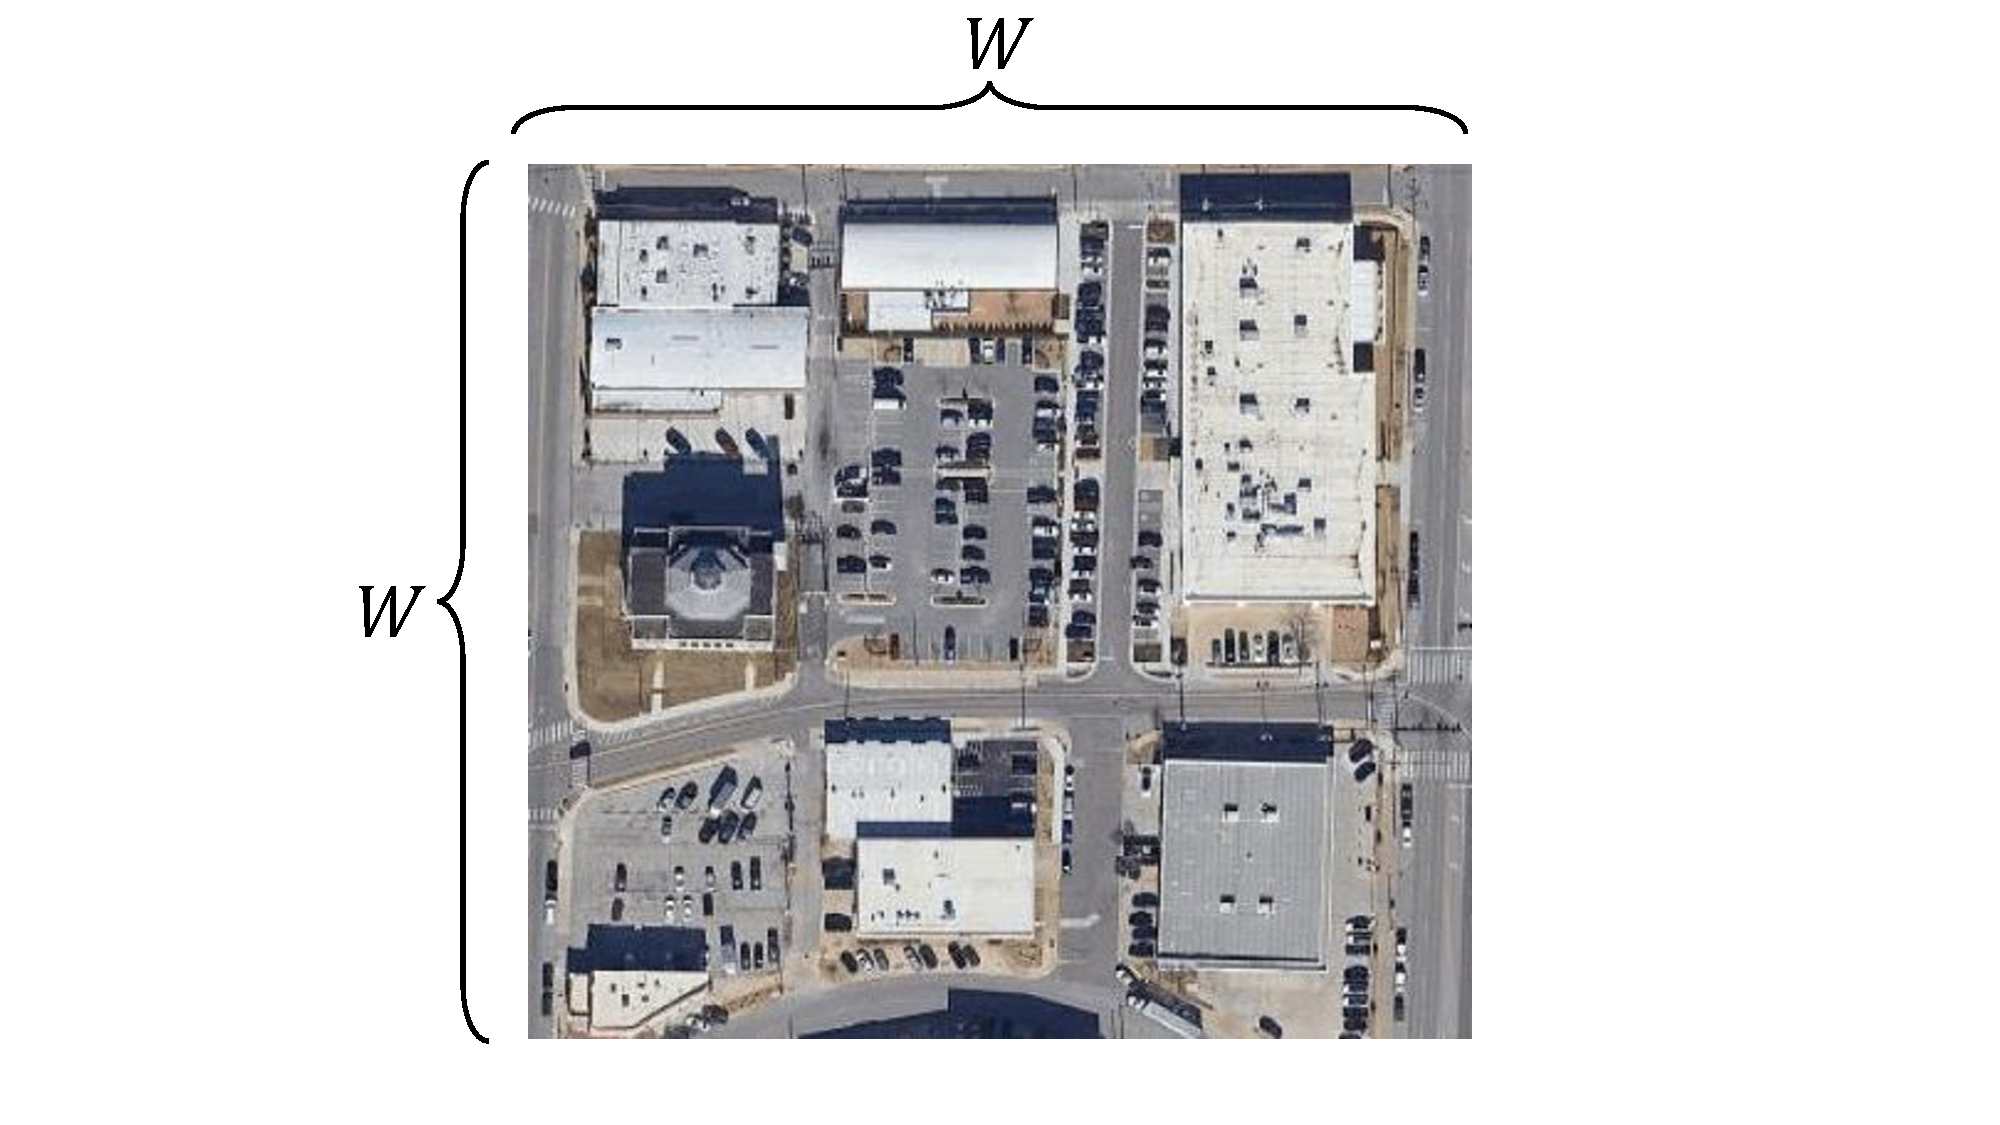
\includegraphics[width=0.8\linewidth]{scenario-a.pdf}
    
    \subcaption{A section of {\it Oklahoma}.}\label{fig:a}
  \end{minipage}
  \hfill
  \begin{minipage}[t]{0.54\linewidth}
    \centering
    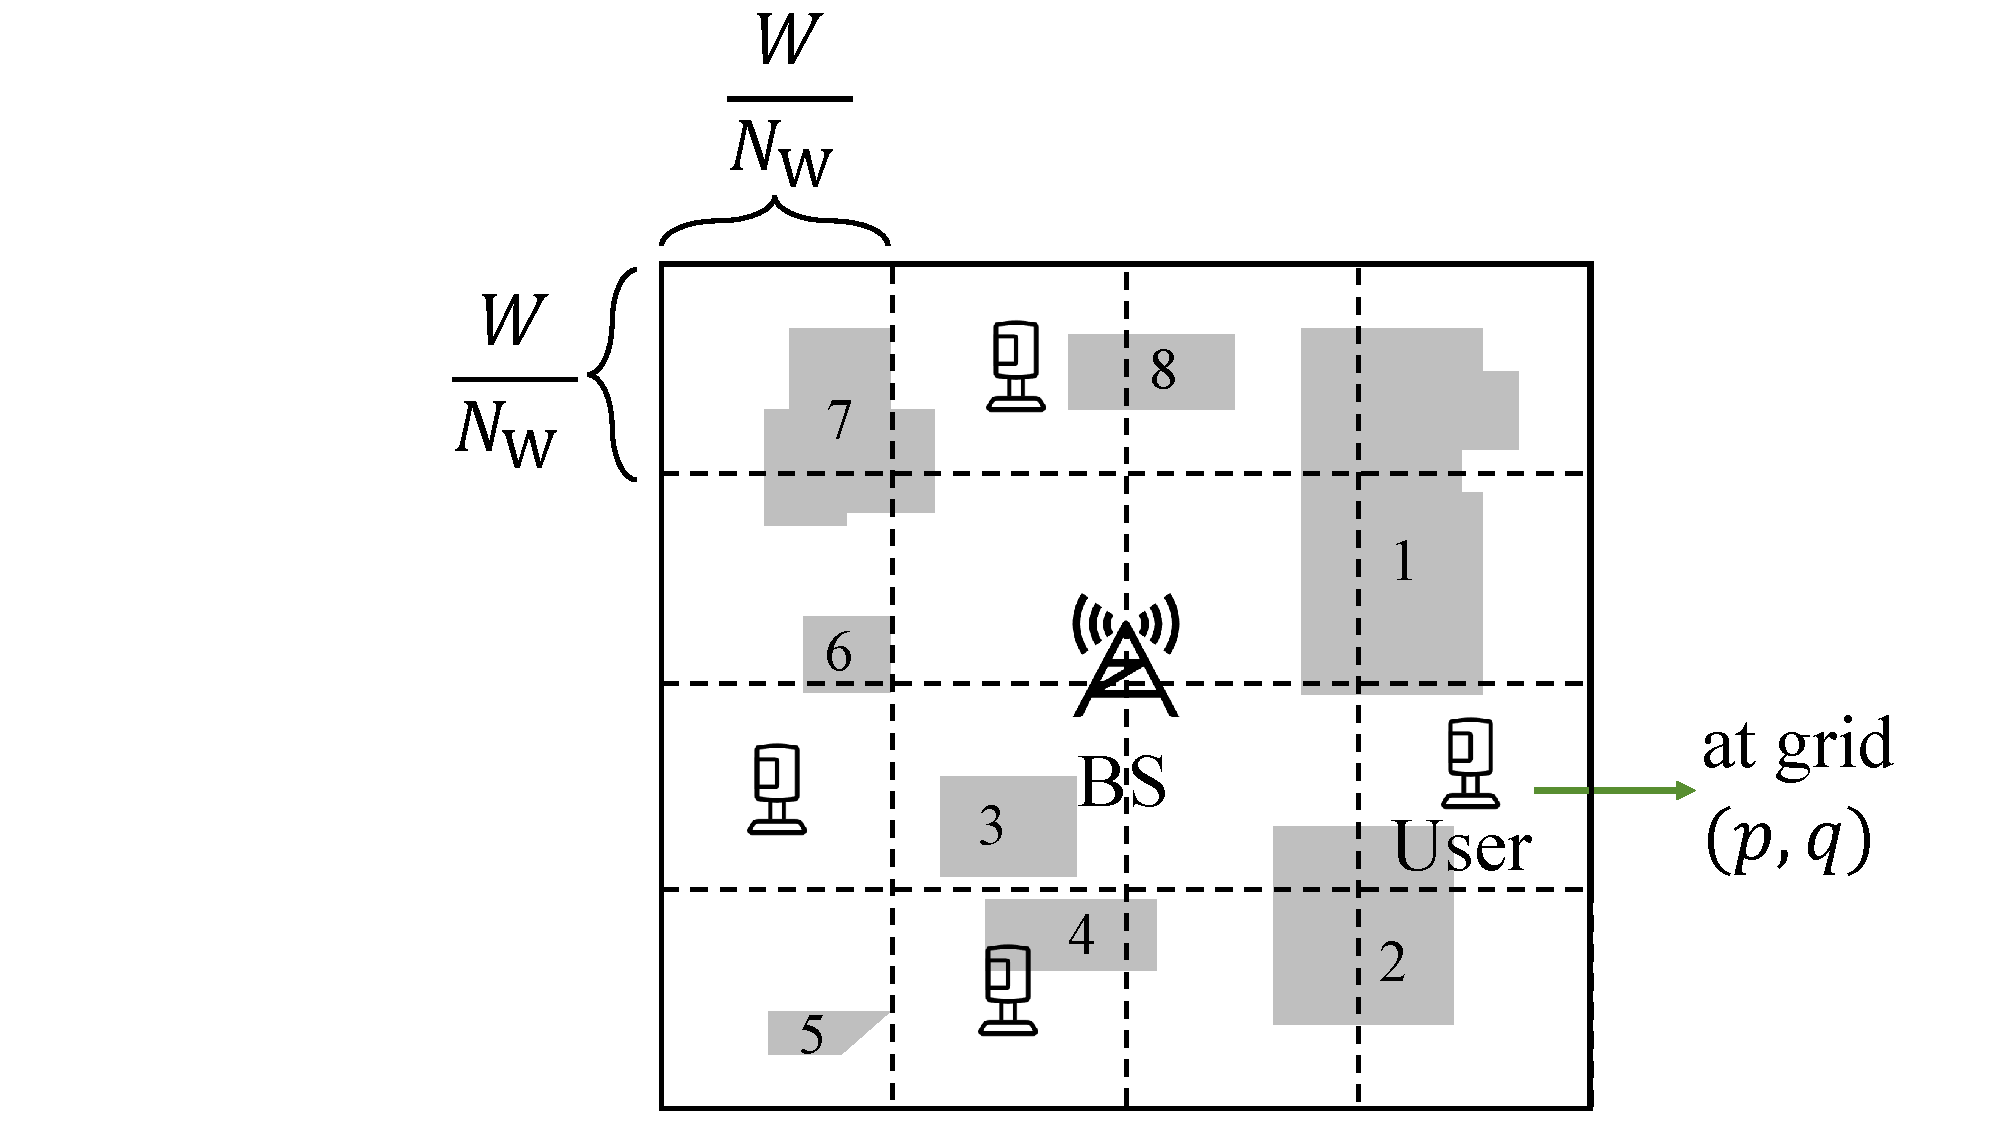
\includegraphics[width=0.9\linewidth]{scenario-b.pdf}
    \subcaption{The schematic diagram.}\label{fig:b}
  \end{minipage}
  \caption{An example scenario for the considered 2D area.}
  \label{new_scenario}
\end{figure}


\subsection{System Model}

We partition the considered 2D area into $N_{\WR} \times N_{\WR}$ grids. A mmWave/THz BS is located at the center of the area, and $K$ users are randomly distributed at the centers of $K$ grids, where these grid centers are not occupied by obstacles, as shown in Fig.~\ref{new_scenario}(b). The BS is equipped with a directional antenna and performs beam scanning over $N_{\dR}$ evenly spaced beams, while each user employs an omnidirectional antenna for reception. 

% For a given environment $\IC$, the channel impulse response (CIR) to a certain user can be given by~\cite{ning2023beamforming}
% \begin{align}
% h_{n}(t)=\sum_{l=1}^{L_{n}} \sqrt{\alpha_{l,n} G_{l,n}^{\tx}G_{l,n}^{\rx}} e^{-j \phi_{l,n}} \delta\left(t-\tau_{l,n}\right),		
% \label{Model_1}
% \end{align} where $t$ is index of time snapshot and $L_{n}$ is the number of paths w.r.t. to the $n$-th beam direction. $\alpha_{l,n}$, $\tau_{l,n}$, $\phi_{l,n}$, $G_{l,n}^{\tx}$, and $G_{l,n}^{\rx}$ are the path gain, delay, phase shift, the transmit and receive antenna gains of the $l$-th path w.r.t. to the $n$-th beam, respectively. Notably, this CIR model is capable of representing key characteristics of mmWave/THz channels, such as non-negligible molecular absorption and channel sparsity. =\!\sum_{l=1}^{L_{n}} \alpha_{l,n} G_{l,n}^{\tx}G_{l,n}^{\rx}


For a given environment $\IC$, the channel impulse response (CIR) is capable of representing key characteristics of mmWave/THz channels, such as non-negligible molecular absorption and channel sparsity~\cite{ning2023beamforming}. Let $h_{p,q,n,\IC}(t)$ denote the CIR to a user located at the center of grid $(p,q)$ under the $n$-th beam direction, where $t$ denotes the time index. The average channel power gain $\bar{h}_{p,q,n,\IC}$ can be expressed as 
\begin{align}
\bar{h}_{p,q,n,\IC}=\frac{1}{T} \int_{0}^{T} |h_{p,q,n,\IC}(t)|^{2} \dR t,		
\label{Model_2}
\end{align}where $T$ represents the total observation time. By averaging the received signal power measured at different times within $T$, we can empirically obtain the average channel power gain $\bar{h}_{p,q,n,\IC}$. As such, channel gains collected from $K$ sparsely distributed users can be obtained. 

To provide a spatial structure, we represent the $K$ channel gains as a sparse tensor $\HF_{\IC}\in\mathbb{R}^{N_{\WR}\times N_{\WR}\times N_{\DR}}$, whose $(p,q,n)$-th entry equals $\bar{h}_{p,q,n,\IC}$ if a user is located in grid $(p,q)$, and $0$ otherwise. Importantly, since the spatial distribution of channel gains is governed by the underlying propagation process, $\HF_{\IC}$ inherently embeds multi-level environmental semantics, making it a natural source of RF observations for sensing.


\begin{figure*}[!t]
\centering
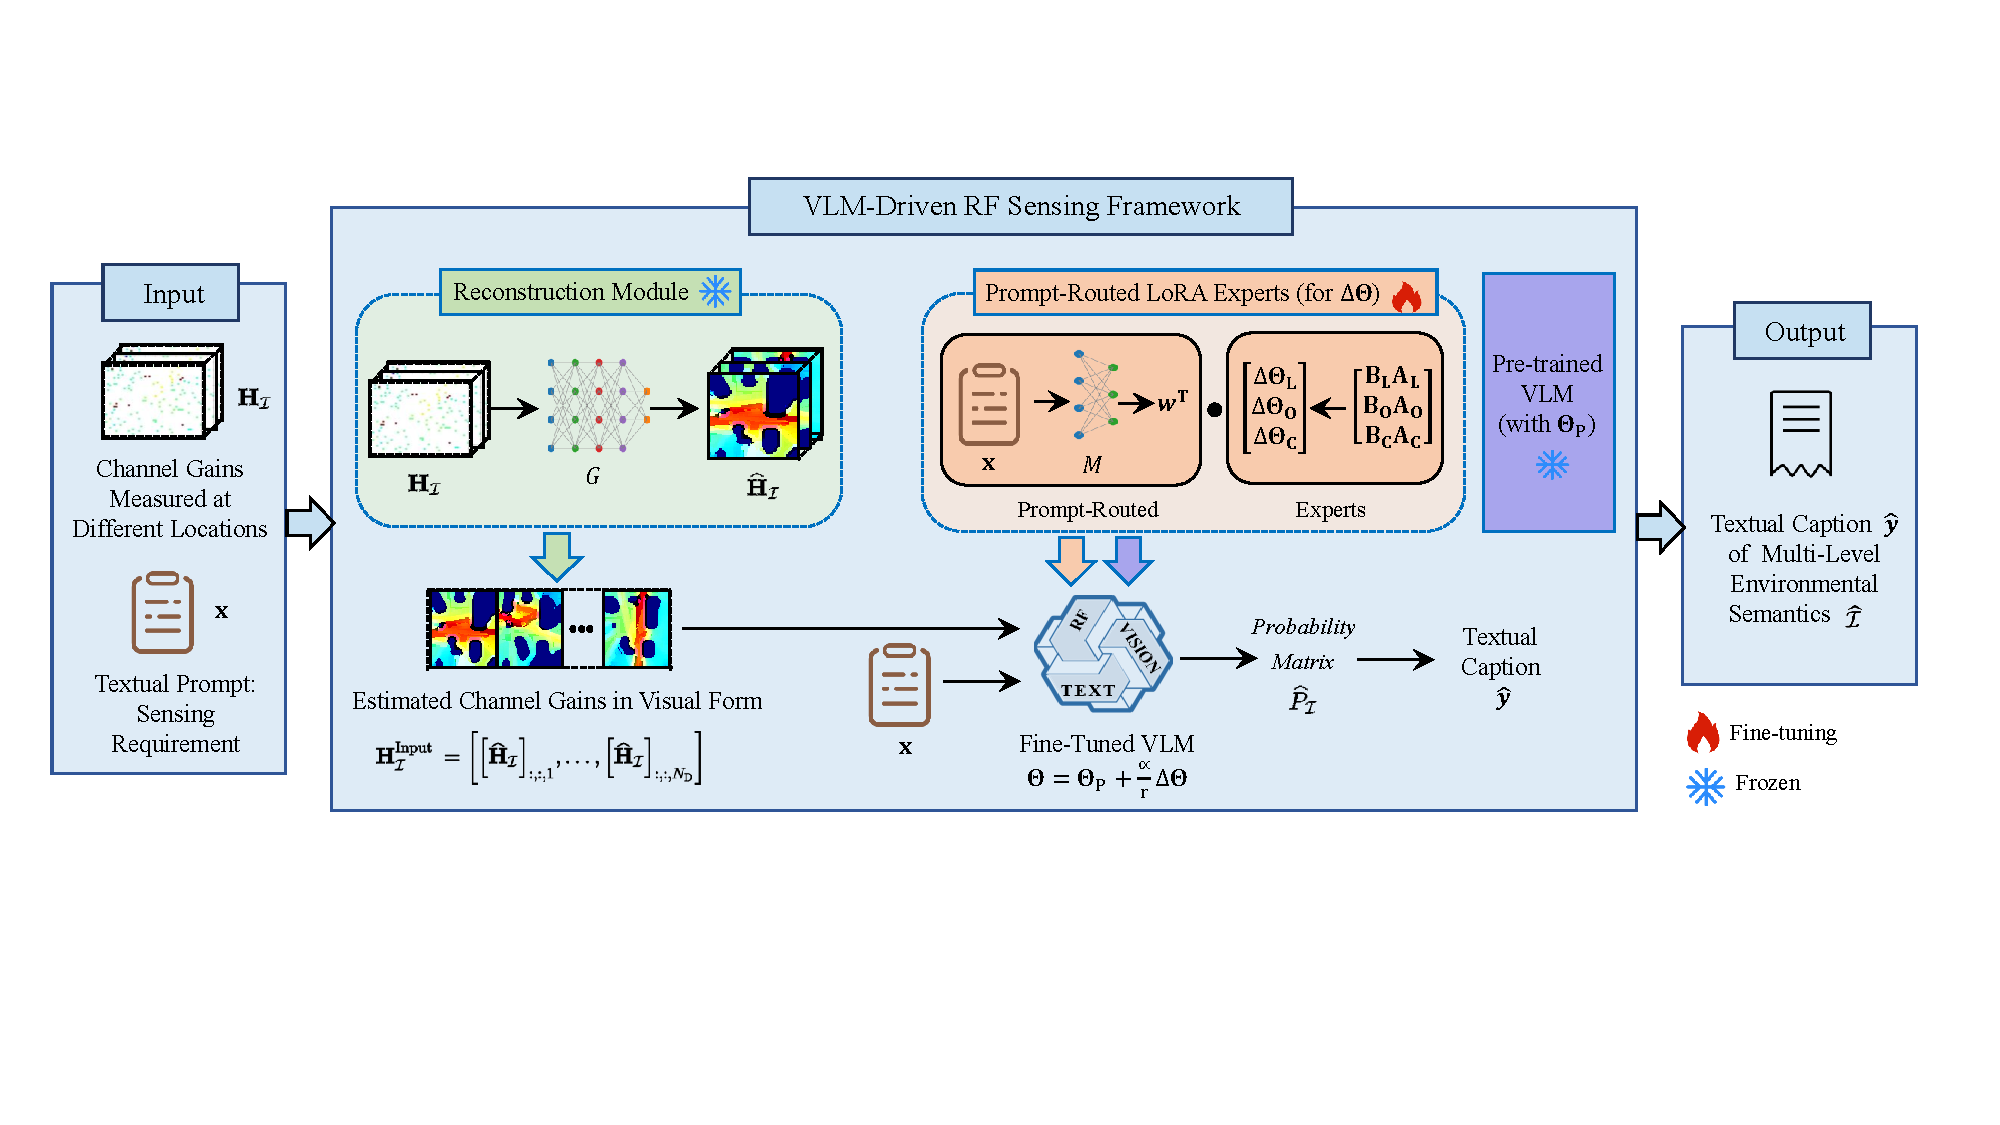
\includegraphics[width=1\linewidth] {framework_final_2.pdf} 

\caption{\centering The proposed VLM-driven RF sensing framework.}
\label{overall_framework}
\end{figure*}

\section{VLM-Driven RF Sensing Framework}


In this section, we propose a task-unified multi-level RF sensing framework driven by VLMs, which captures the environmental semantics $\IC$ from channel gains $\HF_{\IC}$ conditioned on sensing task requirements, as illustrated in Fig.~\ref{overall_framework}. 

\subsection{Problem Formulation}

Motivated by the prompt-conditioned semantic generation capability of VLMs, the proposed framework casts the RF sensing problem as a captioning task, thereby enabling a unified paradigm for diverse sensing tasks. Specifically, the captioning task introduces textual prompts to specify sensing requirements, and generates corresponding environmental captions from RF-domain channel gains. Such a generative formulation not only allows sensing requirements to vary flexibly, but also renders the output space compositional, enabling captions with flexible length, content richness, and semantic levels. In contrast, discriminative formulations adopted by existing methods are restricted to specific sensing requirements and impose a fixed output space.



%(\wh{y}_1,\ldots,\wh{y}_{N_{\yR}'})


Given a pre-defined token vocabulary $\VF$ and a textual prompt represented as a token sequence $\xB\in\VF^{N_{\xR}}$, we define a probability generation function $f\!:\! \Rb^{N_{\WR}\times N_{\WR}\times N_{\DR}} \!\times\! \VF^{N_{\xR}}\!\!\to\!\! [0,1]^{N_{\yR}'\times|\VF|}$ that outputs a probability matrix $\wh{\PB}_{\IC}=f(\HF_{\IC},\xB)$ for the environment with $\IC$. Each row of $\wh{\PB}_{\IC}$ corresponds to a token position and forms a probability distribution over $\VF$.  By maximum-probability decoding from $\wh{\PB}_{\IC}$, we can obtain a token sequence $\wh{\yB}\in\VF^{N_{\yR}'}$, i.e., the generated environmental caption. In other words, the proposed framework generates captions via a probability distribution over $\VF$, where the $j$-th row $[\wh{\PB}_{\IC}]_{j,:}$ corresponds to the token $[\wh{\yB}]_{j}$. 

%Notably, discrete token generation is avoided, since it is non-differentiable and incompatible with gradient-based optimization.

Assuming a ground-truth caption $\yB\in\VF^{N_{\yR}}$ of environmental semantics $\IC$\footnote{For example, an instance of $\IC$ can be described as “this scene contains seven obstacles, each of which is rectangular,” and then tokenized into $\yB$.}, with a corresponding row-wise one-hot matrix $\PB_{\IC}\in\{0,1\}^{N_{\yR}\times|\VF|}$, the captioning problem for RF sensing is formulated as follows:
\begin{subequations}\label{construction}
\begin{align}
	\underset{f}{\mathrm{minimize}}~~&\mathbb{E}_{\IC}\!\left[\LC\left(\wh{\PB}_{\IC},\PB_{\IC}\right)\right], \label{const:2a} \\
	\text{s.t.}~~& \wh{\PB}_{\IC}=f(\HF_{\IC},\xB), \label{const:2d}\\
	& \wh{\PB}_{\IC}\oneF=\oneF, \label{const:2f}\\
	& \PB_{\IC}=g(\IC). \label{const:2b}
\end{align}
\end{subequations} The cross-entropy loss $\LC(\wh{\PB}_{\IC},\PB_{\IC})$ is employed, as it corresponds to maximum likelihood estimation of the token distribution and effectively penalizes deviations from the ground-truth one-hot targets. The mapping $g(\IC)=g_1(g_2(\IC))$ consists of: $g_2(\IC)$ verbalizing $\IC$ into a narrative token sequence $\yB$, and $g_1(\yB)$ converting $\yB$ into $\PB_{\IC}$ by assigning each token in $\yB$ to a one-hot vector over $\VF$.


At the same time, solving problem~\eqref{construction} remains challenging due to the following issues. First, the limited RF prior information, together with the high dimensionality of the obstacle attribute space, may result in an excessively large feasible solution space. Second, a substantial level-dependent gap exists between RF representations and the multi-level linguistic semantics of the environment. Different semantic levels rely on distinct aspects of prior RF knowledge, making a single adaptation path prone to suboptimal alignment for some levels. To mitigate the above challenges and solve problem~\eqref{construction}, we carefully design the framework architecture and fine-tuning strategy based on a pre-trained VLM, as detailed in the following subsections.

\subsection{Framework Architecture}

The proposed framework consists of a pre-trained VLM, a reconstruction module, and three prompt-routed LoRA experts corresponding to the layout, obstacle, and communication-related levels. The framework takes the channel gains $\HF_{\IC}$ and textual prompt $\xB$ as input, and first implements the function $f$ to produce $\wh{\PB}_{\IC}$. Then, by maximum-probability decoding, we obtain the textual caption $\wh{\yB}$, which is embedded with the sensed multi-level environmental semantics $\wh{\IC}=\{\wh{\FIF}_{\LR},\wh{\FIF}_{\ROR},\wh{\FIF}_{\CR}\}$. By leveraging the VLM’s  embedding matrix to compute semantic similarity, $\wh{\IC}$ can be parsed from $\wh{\yB}$. Note that the framework primarily focuses on learning the function $f$, as the mapping from $\wh{\PB}_{\IC}$ to $\wh{\yB}$ or $\wh{\IC}$ follows the aforementioned deterministic procedure.


Benefiting from large-scale pre-training on text–image data, the pre-trained VLM learns powerful visual and textual representations enriched with extensive semantic knowledge. Such properties make VLM well-suited as the backbone of the proposed framework for alleviating the aforementioned challenges in problem~\eqref{construction}. Specifically, their implicit knowledge of real-world spatial structures can be leveraged to constrain the feasible solution space. Meanwhile, the RF-domain channel gains $\HF_{\IC}$ can be represented as images and fed into the VLM, thereby enabling the extraction of informative features via its visual representation capabilities.



The reconstruction module serves to enhance RF priors and further reduce the feasible solution space under sparse observations $\HF_{\IC}$. This module employs a pre-trained network $G$ with parameters $\theta_{\GR}$~\cite{hu2025advancing} to transform $\HF_{\IC}$ into a complete tensor, i.e., $\wh{\HF}_{\IC}=G(\HF_{\IC};\theta_{\GR})$, which provides auxiliary channel gain estimates over unmeasured grids. Then, we concatenate the $N_{\DR}$ slices of $\wh{\HF}_{\IC}$ and transform them into an image, yielding the estimated channel gains in visual form, denoted by $\HF_{\IC}^{\mathrm{Input}}=\big[[\wh{\HF}_{\IC}]_{:,:,1},\ldots,[\wh{\HF}_{\IC}]_{:,:,N_{\DR}}\big]\in\mathbb{R}^{N_{\WR}\times N_{\DR}N_{\WR}}$, which is used as the visual input to the VLM.

To address the level-dependent RF–VLM prior mismatch in a pre-trained VLM, we propose prompt-routed LoRA experts within the framework. This module leverages the level information contained in the prompt $\xB$ to perform a weighted combination of RF sensing knowledge from three LoRA experts at their respective semantic levels. Specifically, the LoRA experts are parameterized by $\Delta\mathbf{\Theta}'=[\Delta\mathbf{\Theta}_{\LR},\Delta\mathbf{\Theta}_{\ROR},\Delta\mathbf{\Theta}_{\CR}]^{\TR}$, where RF sensing knowledge is learned via LoRA-based fine-tuning (see the following subsection) and implicitly encoded in these parameters. A weight vector $\wB$ is generated by a two-layer neural network $M$ with parameters $\theta_{\MR}$~\cite{liu2024moe}, taking the embedding $\xB_{\mathrm{e}}$ of the prompt $\xB$ as input\footnote{The embedding $\xB_{\mathrm{e}}$ is obtained by mapping the prompt $\xB$ through a pre-trained embedding matrix~\cite{bai2025qwen2}.}. As a result, the parameter update $\Delta\mathbf{\Theta}=M(\xB_{\mathrm{e}};\theta_{\MR})^{\TR}\Delta\mathbf{\Theta}'=\wB^{\TR}\Delta\mathbf{\Theta}'$.  

With the parameter update  $\Delta\mathbf{\Theta}$ and the pre-trained VLM parameters $\mathbf{\Theta}_{\PR}$, the parameters of the fine-tuned VLM are given by $\mathbf{\Theta}=\mathbf{\Theta}_{\PR}+\frac{\alpha}{r}\Delta\mathbf{\Theta}$, where $\alpha$ and $r$ are the scaling factor and rank used in LoRA-based fine-tuning, respectively. 


\subsection{LoRA-based Fine-Tuning}

LoRA-based fine-tuning exploits the low “intrinsic rank”~\cite{hu2022lora} of weight updates to enable parameter-efficient adaptation, which helps bridge the level-dependent gap. For each LoRA expert, $\Delta\mathbf{\Theta}_{i\in \{\LR, \ROR, \CR\}}$ is realized by introducing a low-rank update $\BF_{i}\AF_{i}$, 
which is zero-padded into the full parameter space of the VLM. 
Here, $\BF_{i}\in\mathbb{R}^{a\times \frac{r}{3}}$, $\AF_{i}\in\mathbb{R}^{\frac{r}{3}\times b}$, and $r\ll \min(a,b)$. The optimization of $\BF_{i}$ and $\AF_{i}$, i.e., the LoRA-based fine-tuning of the pre-trained VLM, is carried out using the following empirical objective, 
which is a reformulation of problem~\eqref{construction}:
\begin{subequations}\label{final_construction}
\begin{align}
\underset{\BF',\AF',\theta_{\MR}}{\mathrm{minimize}}~~&
\frac{1}{N_{\SR}}\sum_{s=1}^{N_{\SR}}\LC\!\left(\wh{\PB}_{s,\IC},\PB_{s,\IC}\right) \label{const:3a}\\
\text{s.t.}~~&
[\wh{\PB}_{s}]_{j,:}=f_{\mathbf{\Theta}}\!\left([\wh{\yB}_{s}]_{j}\mid [\wh{\yB}_{s}]_{<j},\HF^{\mathrm{Input}}_{s,\IC},\xB\right), \label{const:3d}\\
&
\mathbf{\Theta}\!=\!\mathbf{\Theta}_{\PR}+\frac{\alpha}{r}M(\xB_{\mathrm{e}};\theta_{\MR})^{\TR}d(\BF',\AF'), \label{const:3r}
\end{align}
\end{subequations} where $\BF'=[\BF_{\LR},\BF_{\ROR},\BF_{\CR}]^{\TR}$, $\AF'=[\AF_{\LR},\AF_{\ROR},\AF_{\CR}]^{\TR}$, $j\in\{1,\ldots,N_{\yR}'\}$, and $d(\BF',\AF')$ maps the low-rank matrices in $\BF'$ and $\AF'$ 
to the parameter updates $\Delta\mathbf{\Theta}'$. $N_{\SR}$ is the number of fine-tuning samples. Notably, constraint~\eqref{const:3d} reflects the autoregressive mechanism of the VLM~\cite{bai2025qwen2}, 
under which the output probability matrix $\wh{\PB}_{\IC}$ is generated row by row 
in a prompt-conditioned manner.

%\!\mathbf{\Theta}_{\PR}+\frac{\alpha}{r}\wB^{\TR}\Delta\mathbf{\Theta}'\!=
\section{Experimental Results}
\label{sec:res}

%\subsection{Experimental Setup}

{\bf Datasets and Model Hyperparameters.} We consider three types of 2D scenarios~\cite{hu2025advancing}, which include fine-tuning and validation scenarios with simulated environment, as well as validation scenarios based on the real-world city section shown in Fig.~\ref{new_scenario}(b). These scenarios are labeled as \( \SC_1 \), \( \SC_2 \), and \( \SC_3 \), respectively. When a model is fine-tuned on \( \SC_1 \), scenarios \( \SC_2 \) and \( \SC_3 \) are unseen with respect to that model. Specifically, $\SC_1$ contains $N_{\SR}=1750$ fine-tuning samples from $250$ scenarios, each corresponding to $7$ samples via prompts specifying all combinations of semantic levels. The obstacle numbers in $\SC_1$ are drawn from ${1,2,3,4,5}$, with $50$ scenarios per case. $\SC_2$ contains $350$ validation samples from $50$ scenarios, each with $6$ obstacles. $\SC_3$ contains $56$ validation samples from $8$ scenarios, obtained by sequentially removing obstacles according to their indices in Fig.~\ref{new_scenario}(b). Each scenario in \( \SC_1\) and \( \SC_2\) contains obstacles with randomly generated quadrilateral shapes and positions. We perform ray tracing to obtain mmWave/THz channel gain observations. Following ~\cite{hu2025advancing}, the default hyperparameters are listed in Table~\ref{tab_evalution}. For the communication-related-level information $\FIF_{\CR}$, we consider $4$ predefined BS locations at the centers of the four quadrants. Note that we use Qwen2.5-VL~\cite{bai2025qwen2} as the pre-trained VLM.


{\bf Baseline Models and Evaluation Metrics.} 
Existing methods are typically tailored to specific sensing tasks and therefore cannot support task-unified and multi-level RF sensing. As baselines, we consider U-NetGAN~\cite{hu2025advancing} for obstacle- and layout-level sensing, ResNet-18~\cite{7780459} for communication-related-level sensing, and  Qwen2.5-VL~\cite{bai2025qwen2} for zero-shot inference across all three semantic levels. U-NetGAN infers $\wh{\FIF}_{\LR}$ and $\wh{\FIF}_{\ROR}$ by post-processing its reconstructed environmental maps (e.g., by counting segmented instances to obtain the number of obstacles), while ResNet-18 predicts $\wh{\FIF}_{\CR}$ via multi-class classification. Direct text comparison between $\yB$ and $\wh{\yB}$ is brittle because different words can convey the same environmental semantics. We therefore adopt the averaged macro-F1 score~\cite{11200914} to evaluate the sensed information $\wh{\IC}=\{\wh{\FIF}_{\LR},\wh{\FIF}_{\ROR},\wh{\FIF}_{\CR}\}$, where a higher F1 score indicates better sensing performance in terms of precision and recall. For $\wh{\FIF}_{\LR}$ and $\wh{\FIF}_{\ROR}$, whose attributes are represented in a one-hot manner, the F1 score reduces to the inner product, i.e., $\frac{1}{N_{1}N_{\SR}}\langle\operatorname{vec}(\FIF_{\LR}), \operatorname{vec}(\wh{\FIF}_{\LR})\rangle$ and $\frac{1}{N_{1}N_{3}N_{\SR}}\langle\operatorname{vec}(\FIF_{\ROR}), \operatorname{vec}(\wh{\FIF}_{\ROR})\rangle$, where $\operatorname{vec}(\cdot)$ denotes the vectorization operation. For $\wh{\FIF}_{\CR}$, the F1 score is given by $\frac{1}{N_{1}N_{\SR}}\sum_{s}^{N_{\SR}}\sum_{c}^{N_{1}}\frac{2\langle [\wh{\FIF}_{\CR}]_{c,:},[\FIF_{\CR}]_{c,:}  \rangle}{\left\|[\wh{\FIF}_{\CR}]_{c,:}\right\|_1+\left\|[\FIF_{\CR}]_{c,:}\right\|_1}$.

\renewcommand{\arraystretch}{1.3}   % 行距
\setlength{\tabcolsep}{5pt}          % 列间距

\begin{table}[htbp]
\centering
\caption{Scenario Details and Model Hyperparameters.}
\label{tab_evalution}

\begin{tabular}{
  >{\centering\arraybackslash}p{0.18\textwidth}|
  >{\centering\arraybackslash}p{0.27\textwidth}}\hline
\textbf{Description} & \textbf{Value} \\\hline
Area size & $W\times W=100\,\mathrm{m}\times100\,\mathrm{m}$ \\\hline
Grid division & $N_{\WR}\times N_{\WR}=64\times64$ \\\hline
Number $N_{\SR}$ of samples
  & $\SC_1$: $1750$; $\SC_2$: $350$; $\SC_3$: $56$ \\\hline
Carrier frequency & $300\,\mathrm{GHz}$ \\\hline
Number of beams & $N_{\DR}=18$ \\\hline
Number of users & $K=150$  \\\hline
Learning rate & $0.0001$ \\\hline
Scaling factor and rank & $\alpha=48$ and $r=24$ \\\hline
\end{tabular}
\end{table}

\begin{figure}[!t]
\center
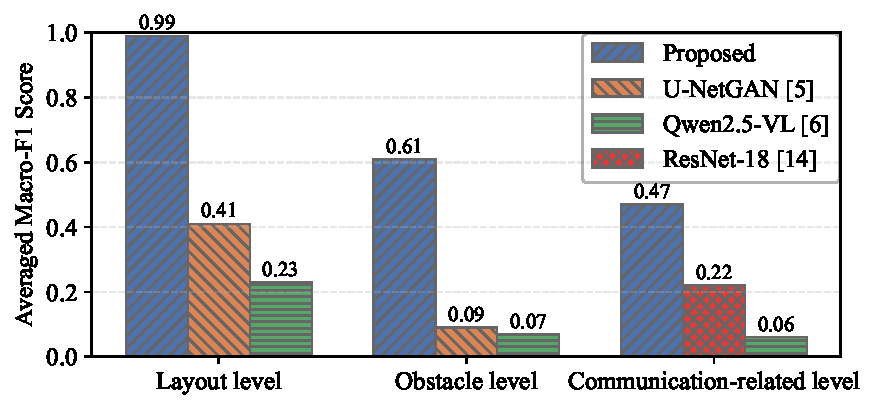
\includegraphics[width=\linewidth] {letter_1.pdf}
\caption{Averaged macro-F1 scores for multi-level environmental semantics sensed by different methods in $\SC_2$.}
\label{ALL_obstacle_RFOB}
\end{figure}


\begin{figure*}[!t]
  \centering
  % 第一行
  \begin{subfigure}[b]{0.30\textwidth}
    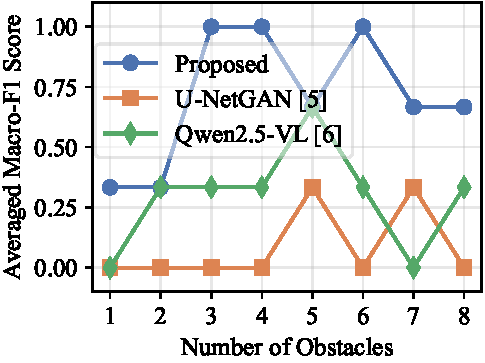
\includegraphics[width=\linewidth]{fig1_layout.pdf}
    \vspace{-1.5em}
    \caption{Layout Level}
    \label{all_GT}
  \end{subfigure}
  \hfill
  \begin{subfigure}[b]{0.30\textwidth}
    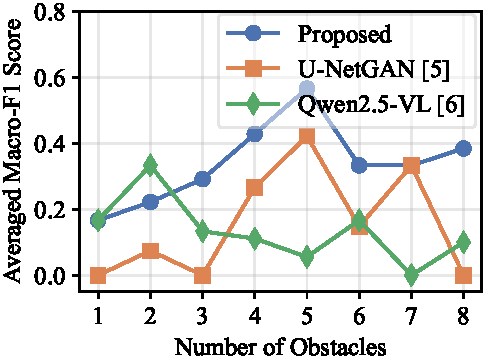
\includegraphics[width=\linewidth]{fig2_obstacle.pdf}
    \label{all_231}
    \vspace{-1.5em}
    \caption{Obstacle Level}
  \end{subfigure}
  \hfill
  \begin{subfigure}[b]{0.30\textwidth}
    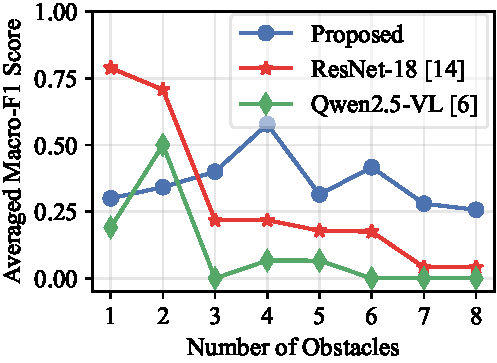
\includegraphics[width=\linewidth]{fig3_comm.pdf}
    \label{all_236}
    \vspace{-1.5em}
    \caption{Communication-Related Level}
  \end{subfigure}
  \caption{Averaged macro-F1 scores versus the number of obstacles for different methods in $\SC_3$.}
  \label{ALL_obstacle}
\end{figure*}

%\subsection{Overall Performance}

Fig.~\ref{ALL_obstacle_RFOB} reports the averaged macro-F1 scores for multi-level environmental semantics sensed by different methods in $\SC_2$. The proposed framework consistently outperforms all baselines across the layout, obstacle, and communication-related levels. In particular, the framework achieves a near-perfect F1 score at the layout level, indicating its strong capability in capturing global structural information. This experiment, conducted in unseen simulated scenarios, demonstrates the effectiveness of the framework, which leverages the RF sensing knowledge from the LoRA experts.

%, yielding up to a 142\% relative improvement over U-NetGAN~\cite{hu2025advancing}
%\subsection{task-unified Generalization Study}
Under the scenarios \( \SC_{3} \), we investigate the impact of the number \( N_{\IR} \) of obstacles on the proposed framework and the baselines, as shown in Fig.~\ref{ALL_obstacle}. The proposed framework achieves higher F1 scores than the baselines in more complex scenarios, i.e., when  \( N_{\IR}>2 \), likely due to the model's enhanced understanding of multiple obstacles, their interactions, and their relationship with communication after adaptation. In the most complex scenario (i.e., \( N_{\IR}=8 \)), the proposed framework achieves an average F1 score improvement of 0.28 across the three levels compared to the baselines

%an average improvement of 176\% across the three levels compared with the baselines.

In Table~\ref{tab_integration_new}, we compare the F1 scores of different methods in $\SC_3$ on an unseen sensing requirement not involved during fine-tuning, where the VLM is prompted to infer possible beam directions for a BS at the scenario center. As shown in Table~\ref{tab_integration_new}, the proposed framework achieves substantially higher performance than the baseline for different obstacle numbers, with an average F1 score improvement of 0.31. Compared with Fig.~\ref{ALL_obstacle}, the different F1 score trend may be attributed to the increased generalization difficulty and uncertainty across both unseen scenarios and requirements. ResNet-18~\cite{7780459} is excluded as it is not trained for this requirement, whereas the proposed framework remains applicable, demonstrating the advantage of the task-unified RF sensing paradigm.




\renewcommand{\arraystretch}{1.3}   % 行距
\setlength{\tabcolsep}{6pt} 
\begin{table}[ht]
\centering
\caption{F1 Score Comparison on an Unseen Sensing Requirement.}
\label{tab_integration_new}

\begin{tabular}{|
  >{\centering\arraybackslash}m{0.109\textwidth}|
  >{\centering\arraybackslash}m{0.02\textwidth}|
  >{\centering\arraybackslash}m{0.02\textwidth}|
  >{\centering\arraybackslash}m{0.02\textwidth}|
  >{\centering\arraybackslash}m{0.02\textwidth}|
  >{\centering\arraybackslash}m{0.02\textwidth}|
  >{\centering\arraybackslash}m{0.02\textwidth}|
  >{\centering\arraybackslash}m{0.02\textwidth}|
  >  {\centering\arraybackslash}m{0.02\textwidth}|}
\hline

\multirow[c]{2}{*}{\textbf{Method}} 
& \multicolumn{8}{c|}{\textbf{Number of obstacles in $\SC_3$}} \\ \cline{2-9}
& \textbf{1} & \textbf{2} & \textbf{3} & \textbf{4} & \textbf{5} & \textbf{6} & \textbf{7} & \textbf{8} \\
\hline

% ---------- Loss Function ----------

\textbf{Proposed} & 0.77 & 0.55 & 0.40 & 0  & 0.40 & 0.22 & 0.22 & 0.22 \\\hline

\textbf{Qwen2.5-VL~\cite{bai2025qwen2}}  & 0.29 & 0 & 0 & 0 & 0 & 0 & 0 & 0  \\
\hline
\end{tabular}
\end{table}

\section{Conclusion}

In this letter, we have proposed a novel framework that adapts VLMs for task-unified multi-level RF sensing. The framework has been designed to process mmWave/THz channel gains and diverse sensing requirements, generating environmental semantic captions across the layout, obstacle, and communication-related levels. By introducing prompt-routed LoRA experts, it has mitigated the RF–VLM prior mismatch and enabled level-aware adaptation. Simulation results have demonstrated that the framework achieves an F1 score improvement of up to 0.31 over the baselines for RF sensing.

% 参考文献计入的话，感觉参考文献也可以删一些，感觉有点多
\bibliographystyle{IEEEtran}
\bibliography{ref}

\end{document}
